\subsection{Determinação da densidade de um líquido utilizando o
Areômetro de Nicholson}

Da mesma forma que o experimento anterior, utilizaremos o areômetro como instrumento para determinar a densidade, mas agora não de um sólido, mas sim de um líquido. Ele não foi feito inventado para essa finalidade, mas produz ainda sim um resultado aceitável.

\begin{figure}[H]
    \centering
    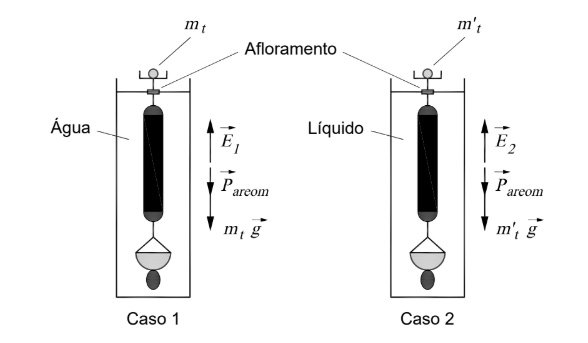
\includegraphics[scale=0.8]{images/aerometro-densidade-liquido.png}
    \caption{Representação do experimento para determinar a densidade de um líquido utilizando um areômetro}
\end{figure}

Para começar, iremos inserir o instrumento numa líquido cujo valor de $\rho$ é conhecido (no caso será água a 25°C). Então colocamos o recipiente com água e taramos a balança, para que agora possamos aflorar o areômetro, anotando o valor da massa do areômetro junto com os pesinhos ($m_{ar} + m_{pa}$). Pesando depois as massinhas separadamente ($m_t$) podemos determinar o valor do volume do areômetro, que será dado fórmula básica da densidade:

\[ V_{ar} = \frac{m_{ar} + m_t}{\rho _{agua}} \]

\[ \delta V_{ar} = \frac{\delta m_{ar} + \delta m_t}{\rho _{agua}} \]

Com esse dado em mão podemos partir para a determinação da densidade do líquido desconhecido. Assim sendo, iremos primeiramente encher a proveta com esse líquido e aflorar o areômetro lá imerso, e pesaremos o valor das massinhas utilizadas ($m_t'$). Com esse valor em mãos, podemos utilizar a fórmula deduzida no vídeo para o cálculo de densidades utilizando um aerômetro:

\[ \rho _x = \rho _{agua} + \frac{m_t - m_t'}{V_{ar}} \]

\[ \delta \rho _x = \rho _{agua} \cdot \frac{(\delta m_t + \delta m_t') \cdot V_{ar} + \delta V_{ar} \cdot (m_t - m_t')}{V_{ar}^2} \]

Após a obtenção de $\rho _x$ vamos utilizar uma tabela online para deduzir o que ele é.
